\documentclass[english,11pt]{beamer}

\DeclareMathOperator{\Cov}{Cov}
\DeclareMathOperator{\Var}{Var}
\DeclareMathOperator{\E}{\mathbb{E}}
\DeclareMathOperator{\Proba}{\mathbb{P}}

\newcommand{\Covb}[2]{\ensuremath{\Cov\!\left[#1,#2\right]}}
\newcommand{\Eb}[1]{\ensuremath{\E\!\left[#1\right]}}
\newcommand{\Pb}[1]{\ensuremath{\Proba\!\left[#1\right]}}
\newcommand{\Varb}[1]{\ensuremath{\Var\!\left[#1\right]}}

% norm
\newcommand{\norm}[1]{\| #1 \|}

\newcommand{\indep}{\rotatebox[origin=c]{90}{$\models$}}





\usepackage{mathptmx,amsmath,amssymb,graphicx,bibentry,bbm,babel,ragged2e}

\makeatletter

\newcommand{\noun}[1]{\textsc{#1}}
\newcommand{\jitem}[1]{\item \begin{justify} #1 \end{justify} \vfill{}}
\newcommand{\sframe}[2]{\frame{\frametitle{#1} #2}}

\newenvironment{centercolumns}{\begin{columns}[c]}{\end{columns}}
%\newenvironment{jitem}{\begin{justify}\begin{itemize}}{\end{itemize}\end{justify}}

\usetheme{Warsaw}
\setbeamertemplate{footline}[text line]{}
\setbeamercolor{structure}{fg=purple!50!blue, bg=purple!50!blue}

\setbeamersize{text margin left=15pt,text margin right=15pt}

\setbeamercovered{transparent}


\@ifundefined{showcaptionsetup}{}{%
 \PassOptionsToPackage{caption=false}{subfig}}
\usepackage{subfig}

\usepackage[utf8]{inputenc}
\usepackage[T1]{fontenc}



\makeatother

\begin{document}


\title{Complexity, Complexities and Complex Knowledges\\
\textit{Discussion of Pr. Batty: ``Complexity in Urban Systems''}
}

\author{J.~Raimbault$^{1,2,\ast}$\\
\texttt{juste.raimbault@polytechnique.edu}
}


\institute{$^{1}$UMR CNRS 8504 G{\'e}ographie-cit{\'e}s\\
$^{2}$UMR-T IFSTTAR 9403 LVMT
}


\date{Geodivercity International Workshop\\\smallskip
12-13th October 2017
}

\frame{\maketitle}





%%%%%%%%%%%%%%%%%%%
%% ABSTRACT

% This discussion aims at exploring the consequences of the existence of different types of complexities in the study of socio-technical systems. We illustrate links between three different type of complexities, namely weak emergence in the sense of~\cite{bedau2002downward}, computational complexity and informational complexity. Emergence and computational complexity are closely linked, as suggested by the computational capabilities of many complex systems.
%The Turing complete properties of many complex systems suggest some cases where emergence implies computational complexity, whereas the recently shown NP-completeness of approximating elementary physical equations~[\cite{2014arXiv1403.7686B}] gives the opposite implication.
% Informational complexity can also been shown to play a crucial role in self-organisation, through spatial patterns of information flows for example.
% We postulate that complex knowledge of socio-technical systems must capture conjointly different types of complexities and their interactions, and that this property is an other expression of a necessary reflexive nature of complex knowledge.





\sframe{More or Less Complex Urban Systems ?}{

\centering

\hspace{-0.3cm}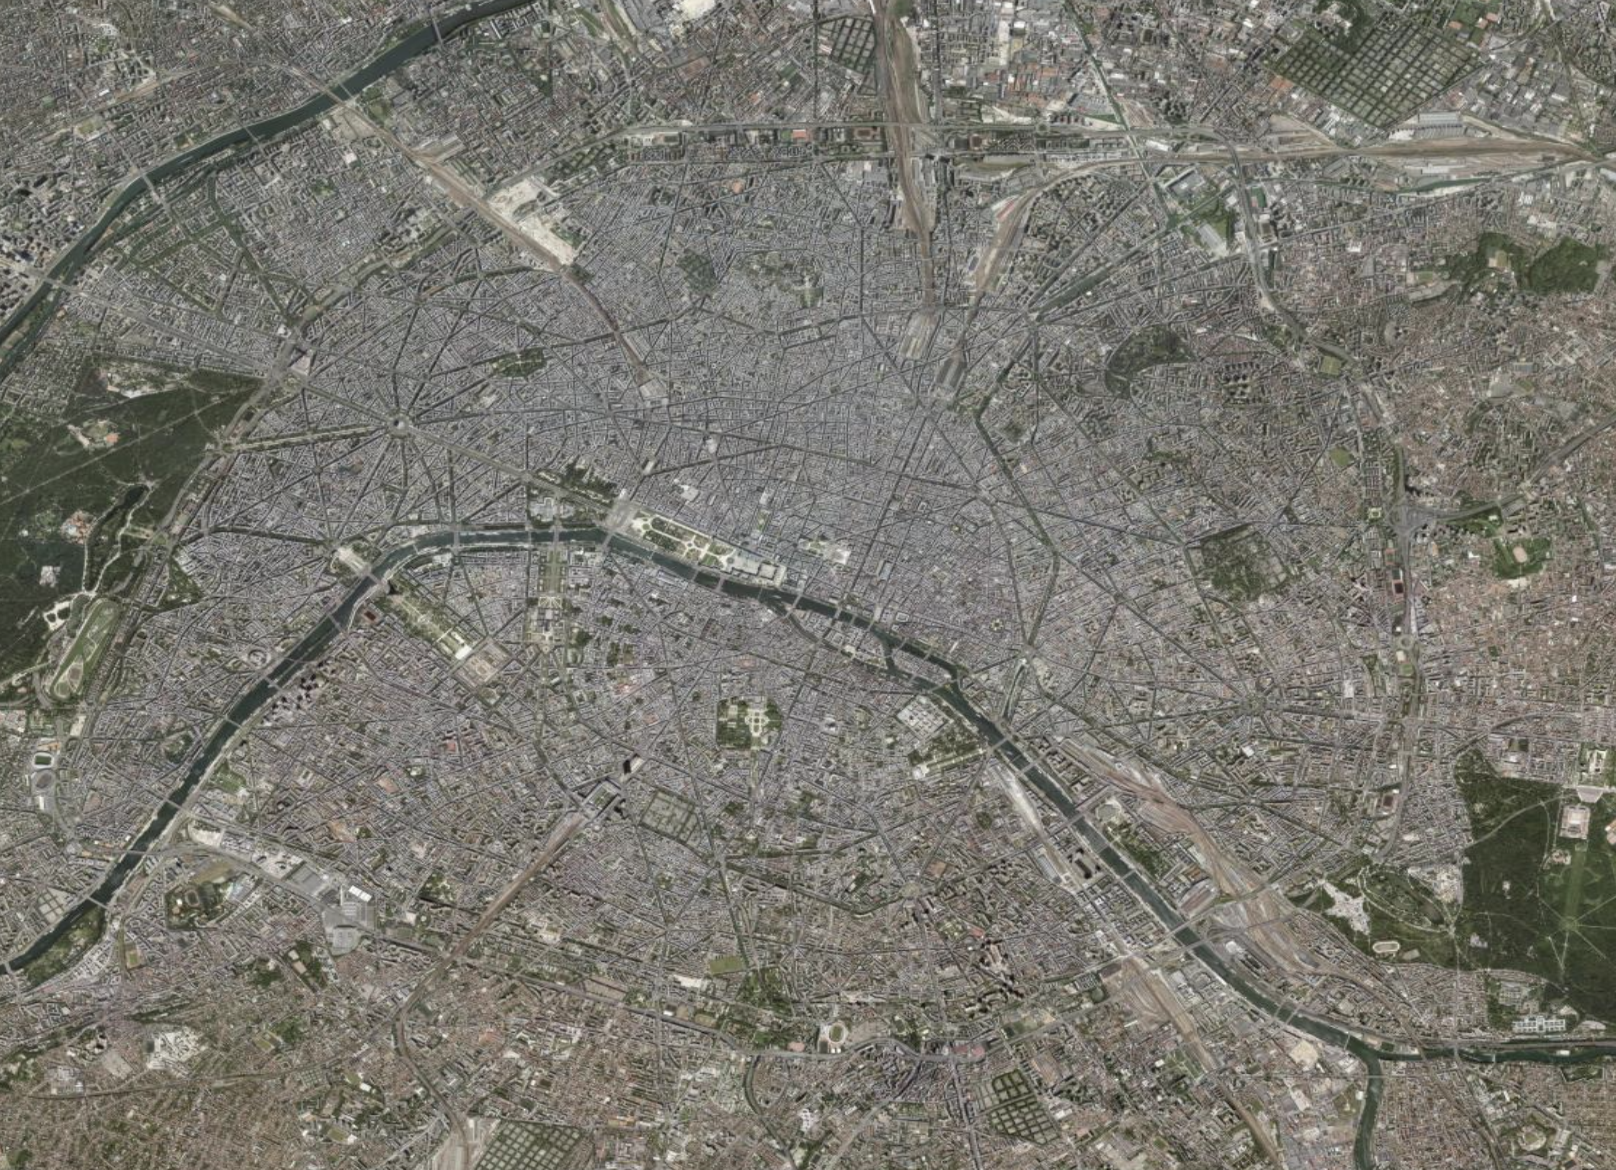
\includegraphics[width=0.54\textwidth]{figures/intro_paname}\hspace{0.3cm}
\includegraphics[width=0.45\textwidth]{figures/intro_barcelone}

\bigskip

\footnotesize\textit{Source: Geoportail, Google maps}
}



\sframe{Some Types of Complexity}{

% definition and question

\justify

\textit{Various approaches to complexity, corresponding definitions, characterizations and measures. We consider:}

\medskip

\begin{itemize}
	\item Complex Systems as systems exhibiting Weak Emergence~\cite{bedau2002downward}
	\item Computational Complexity: $\mathbf{P}\neq \mathbf{NP}$, Algorithmic Complexity\\ (see~\cite{moore2011nature})
	\item Informational Complexity: information theory, Complexity profile~\cite{allen2017multiscale}
\end{itemize}

\medskip

$\rightarrow$ \textit{What are the links between these different types of complexities ?}

}



\sframe{Computational Complexity of Complex Adaptive Systems}{

\justify

\textit{Complex Systems require a minimal level of computational complexity}

\bigskip
\bigskip

$\rightarrow$ \cite{2014arXiv1403.7686B} shows that solving the Schrodinger equation with an arbitrary Hamiltonian is NP-complete

\bigskip

$\rightarrow$ \cite{tovsic2017boolean} gives a lower bound for computational complexity of very simple ABMs when adding interactions with the environment


}



\sframe{Computation by Complex Adaptive Systems}{

\textit{Computation is achieved by diverse Complex Systems}

\medskip

$\rightarrow$ Ant algorithm solves generalized TSP \cite{Pintea2017}

\bigskip

\centering

\frame{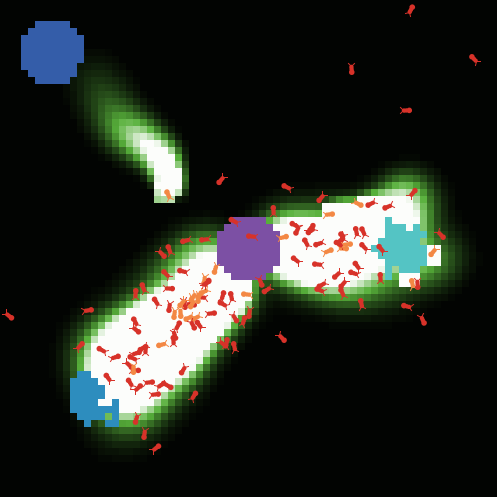
\includegraphics[width=0.31\textwidth]{figures/computation_ants}}\hspace{0.2cm}
\frame{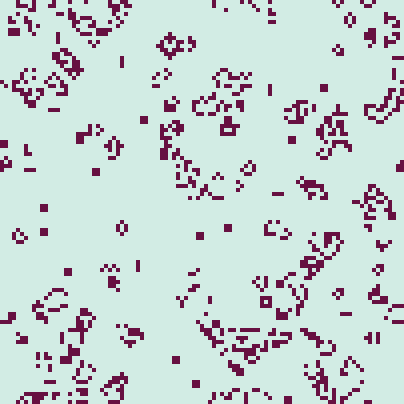
\includegraphics[width=0.31\textwidth]{figures/computation_gameoflife}}\hspace{0.2cm}
\frame{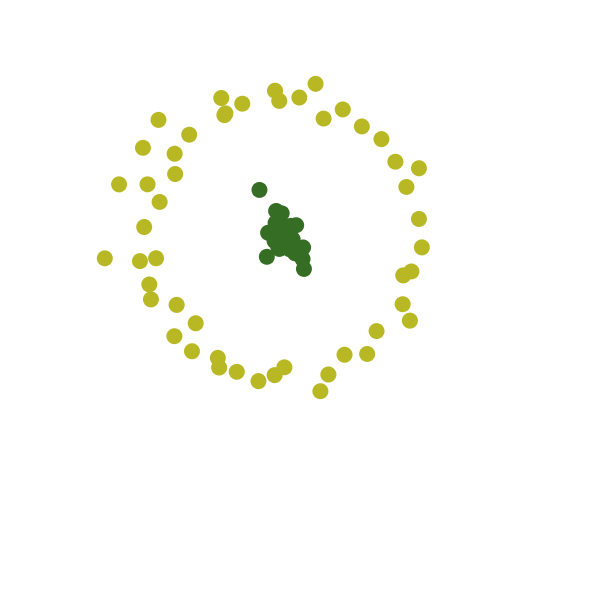
\includegraphics[width=0.31\textwidth]{figures/computation_swarmchem}}\hspace{0.2cm}

\justify

\footnotesize\textit{Sources. Ants, Game of Life: NetLogo Library; Swarm chemistry: implementation of \cite{sayama2007decentralized}}

}


\sframe{Information and Complex Systems}{

% Chua local activity principle ; information storage for life ; Holland signals and boundaries ; School of fishes Emanuele

\textit{Central role of information in Complex Systems}

\medskip

$\rightarrow$ Chua's local activity principle~\cite{mainzer2013local} drives local entropy for some reaction-diffusion systems

$\rightarrow$ Central role of Signals and their processing in Holland's approach to CAS~\cite{holland2012signals}

\bigskip

\centering
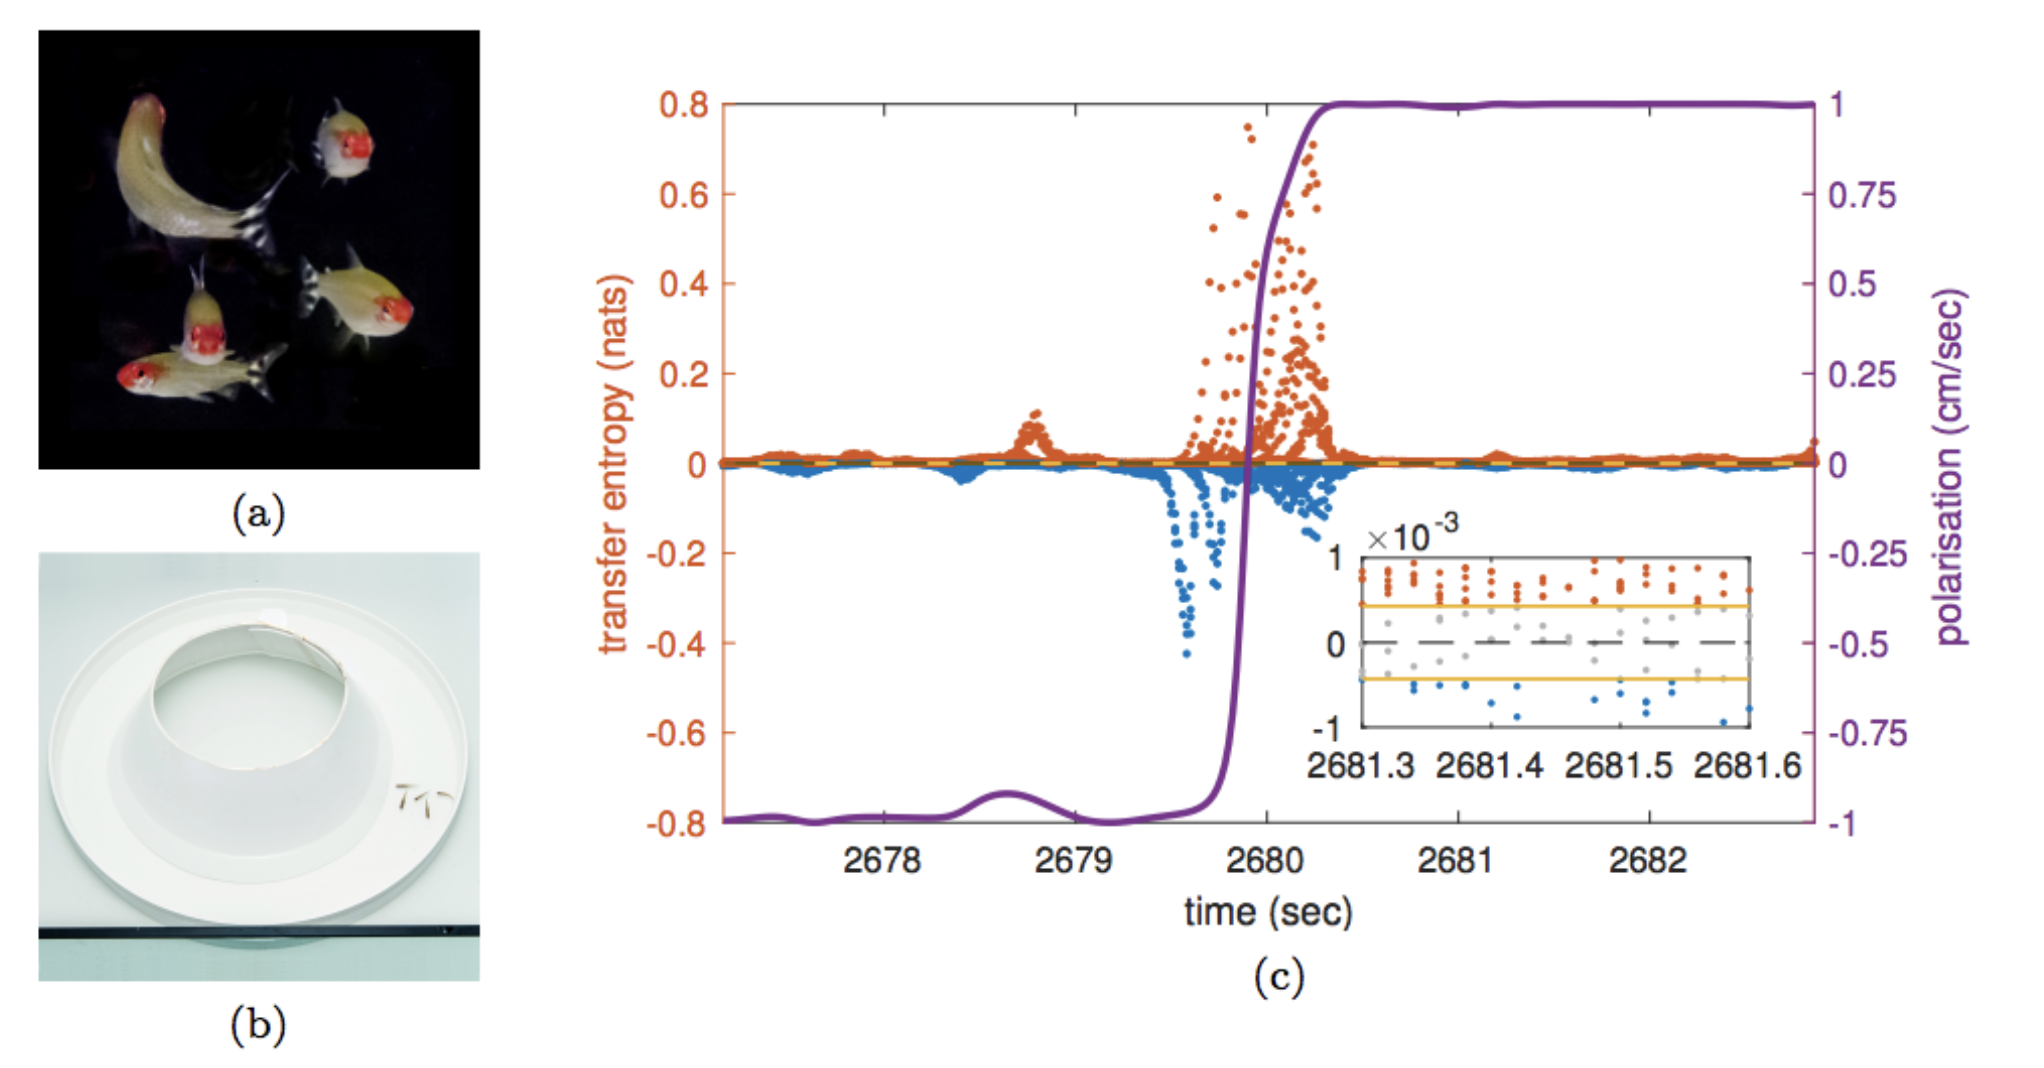
\includegraphics[width=0.7\textwidth]{figures/info_fishschool}

\footnotesize\textit{Role of transfer entropy in collective behavior in a school of fishes, from~\cite{crosato2017informative}}

}


\sframe{Knowledge of the Complex}{

% is complex though, or complex knowledge, the same as knowledge of the complex ? (simple models of cs ? -> cf Control and Cybernetics ! : x principle

\justify

\textit{Given that:}

\begin{enumerate} 
\item \textit{Processes of knowledge production on Complex Systems necessite high level of complexity for each aspect.}

\item \textit{They must translate the different type of complexities, and the relations between these.}
\end{enumerate}

\bigskip

\textbf{Postulate : } Knowledge of the Complex has an inevitable reflexive nature, in the sense of recursive theories (knowledge on producer of the knowledge is part of the knowledge)
% first order recursive functions ?

\bigskip

$\rightarrow$ \textit{Knowledge of the Complex} is thus {Complex Knowledge} (cf law of requisite complexity~\cite{gershenson2015requisite}). Link with an ``Evolutive Rationality'', Complex Knowledge being both the product and the support of its evolution ?

}


\sframe{Conclusion}{

% implications for urban systems ; echo with Batty
% other types of complexity ? (Denise's disciplinary complexity ; knowledge framework)

$\rightarrow$ Non-reflexive approaches will never fully grasp Urban Complexity (or \textit{Social Sciences are necessary})

\bigskip

$\rightarrow$ Extension to other types of complexity such as Pumain's ``disciplinary complexity''~\cite{pumain2005cumulativite} ? \textit{Integrative approaches may be necessary}

\bigskip

$\rightarrow$ Link with Knowledge Domains~\cite{raimbault2017applied}

}




\sframe{Reserve slides}{

\centering

\Large

\textbf{Reserve Slides}

}



%%%%%%%%%%%%%%%%%%%%%
\begin{frame}[allowframebreaks]
\frametitle{References}
\bibliographystyle{apalike}
\bibliography{/Users/juste/ComplexSystems/CityNetwork/Biblio/Bibtex/CityNetwork,biblio}
\end{frame}
%%%%%%%%%%%%%%%%%%%%%%%%%%%%











\end{document}







